% AAAI-27 Demonstration Track submission.
% Requires the official AAAI-27 author kit (aaai27.sty + aaai27.bst); place the
% kit files next to this file and compile:
%   pdflatex aaai27_demo && bibtex aaai27_demo && pdflatex aaai27_demo && pdflatex aaai27_demo
% Track limits: two pages of content plus up to one page of references,
% AAAI two-column style. Single-blind (permitted by the call).
% Structure follows accepted AAAI-25 demo papers (e.g., "Agentic AI for
% Digital Twin", "Bidirectional Human-AI Learning in Real-Time Disoriented
% Balancing"): Figure 1 with a long caption carrying the video link,
% plain section names, numbered demo phases, and a short Conclusion.
\documentclass[letterpaper]{article}
\usepackage{aaai27}
\usepackage{times}
\usepackage{helvet}
\usepackage{courier}
\usepackage[hyphens]{url}
\usepackage{graphicx}
\urlstyle{rm}
\def\UrlFont{\rm}
\usepackage{natbib}
\usepackage{caption}
\usepackage{booktabs}
\usepackage{tikz}
\usetikzlibrary{positioning,arrows.meta}
\frenchspacing
\setlength{\pdfpagewidth}{8.5in}
\setlength{\pdfpageheight}{11in}

\pdfinfo{
/TemplateVersion (2027.1)
}

\title{NH3Bench: Language-Model Shift Engineers\\ on an Ammonia-Plant Digital Twin}
\author{
    Nikolay Nikitin
}
\affiliations{
    nicl.nno@gmail.com\\
    \url{https://github.com/nicl-nno/NH3Bench}
}

\begin{document}

\maketitle

\begin{abstract}
We demonstrate NH3Bench, a benchmark in which a language model acts as the
shift engineer of an industrial ammonia (R717) refrigeration plant simulated
by a physics-based digital twin. The benchmark is accident-forcing (inaction
ends in catastrophe), runs in pseudo-real time (reasoning tokens convert to
virtual seconds, so a correct answer can arrive after the rupture), and is
partially digitalized (part of the truth exists only on local gauges, fetched
by dispatching simulated workers). Across six calibrated scenarios, four
Claude-family models score between 32 and 91 of 100. Attendees watch live
episodes with the models' reasoning streams and play the same scenarios
themselves, under the same clock, in a browser-based trainer running the same
twin.
\end{abstract}

\section{Introduction}

Language-model agents are being proposed for operational roles in physical
industries, yet existing agent benchmarks evaluate them on digital-native
tasks: tool use in software environments \citep{liu2023agentbench},
customer-service dialogues under rule compliance \citep{yao2024tau}, or
procedure following where the correct procedure is supplied in the prompt
\citep{sopbench2025}. Industrial-asset suites stop short of a closed control
loop \citep{assetops2025}, and real-time operator studies use abstract text
simulators without physics \citep{nrtbench2026}. Industrial reality differs
in three ways these settings do not capture: in a developing incident
\emph{doing nothing is itself a decision} with physical consequences; the
plant does not pause while the agent deliberates; and no SCADA system sees
everything---a shift engineer's information set includes sight glasses, local
gauges, smells and sounds, fetched by people at a cost in minutes and,
sometimes, in exposure.

NH3Bench operationalizes all three in a domain with a documented accident
record: the 2010 Millard Refrigerated Services ammonia release was caused by
a defrost cycle interrupted by a power loss \citep{csb2010}---the mechanism
reconstructed in our first scenario. Every outcome is produced by a
thermodynamic model whose mass balance closes to under 0.1\,\% and which
reproduces a Millard-class hydraulic shock (201 bar against a 186 bar pipe
limit).

\begin{figure}[t]
\centering
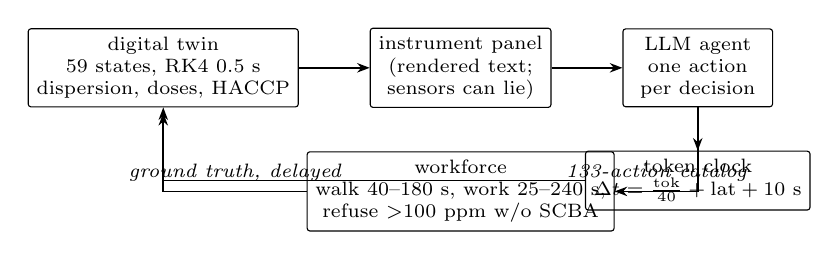
\begin{tikzpicture}[
  font=\scriptsize,
  box/.style={draw, rounded corners=1pt, align=center, inner sep=3pt},
  lbl/.style={font=\scriptsize\itshape, align=center},
  arr/.style={-{Stealth[length=1.6mm]}, semithick}
]
\node[box, minimum width=2.5cm] (twin)
  {digital twin\\59 states, RK4 0.5 s\\dispersion, doses, HACCP};
\node[box, right=0.9cm of twin, minimum width=2.2cm] (obs)
  {instrument panel\\(rendered text;\\sensors can lie)};
\node[box, right=0.9cm of obs, minimum width=1.9cm] (llm)
  {LLM agent\\one action\\per decision};
\node[box, below=0.55cm of obs, minimum width=2.2cm] (wf)
  {workforce\\walk 40--180 s, work 25--240 s,\\refuse $>$100 ppm w/o SCBA};
\node[box, below=0.55cm of llm, minimum width=1.9cm] (clock)
  {token clock\\$\Delta t = \frac{\mathrm{tok}}{40} + \mathrm{lat} + 10$ s};
\draw[arr] (twin) -- (obs);
\draw[arr] (obs) -- (llm);
\draw[arr] (llm) |- node[lbl, pos=0.75, above] {133-action catalog} (wf);
\draw[arr] (wf) -| node[lbl, pos=0.25, above] {ground truth, delayed} (twin);
\draw[arr] (llm) -- (clock);
\draw[arr] (clock) -| ([yshift=-2pt]twin.south);
\end{tikzpicture}
\caption{The NH3Bench loop. The agent sees rendered instrument readings, not
plant state, and answers with one action id from a fixed 133-action catalog:
remote commands, safety systems, or work orders that dispatch one of two
simulated operators. Manual measurements return ground truth, bypassing
failed sensors---in most scenarios SCADA disagrees with reality at least
once. Every reasoning token advances the plant by 1/40 s before the action
executes, so verbosity is a safety variable. A demonstration video will be
available at the repository URL above.}
\label{fig:loop}
\end{figure}

\section{Benchmark Design}

The twin models a 250 t/day dairy plant: four screw compressors on two
suction stages, two evaporative condensers, three vessels, six air coolers,
hot-gas defrost, an ice-water circuit, HACCP-critical product temperatures,
and a dispersion model with per-operator dose accounting.
Figure~\ref{fig:loop} shows the decision loop.

Six scenarios are admitted by a calibration quartet plus an always-ESD
baseline: inaction must end in catastrophe; a scripted oracle must pass
cleanly using only observable evidence; a faithful checklist policy
($\pi_{\mathrm{reg}}$) must fail or pay heavily; random action must not
save. Scenario mechanisms include a hung defrost whose remote abort is
silently swallowed by the stuck sequencer (S1), a loud leak masking a dead
level sensor (S2), an air-in-condenser false trail (S3), and an isolation
trap where the regulation's own reflex causes the rupture (S4). Two
scenarios are \emph{mirrored controls}: S5 punishes over-reaction to a
drifting gas detector, while S6 presents the same evidence picture and then
lets the discredited instrument start telling the truth---the fatal error is
closing the question and never re-opening it. S6 also closes a loophole we
found empirically: an ``emergency-stop everywhere'' meta-policy scores
88.6/100 on S1--S5 with no diagnosis at all, but ends in catastrophe on S6,
where the leak is independent of the compressors.

Alongside Prevention Rate the benchmark reports \emph{Regulation Gap}: score
minus that of the published checklist policy---an agent that cannot beat the
written regulation scores below zero regardless of raw prevention. A unified
0--100 score multiplies independent axes: catastrophe or an incapacitated
worker zeroes the run; operator dose multiplies (never monetized); economics
and discipline fill the remainder. Points of no return, found by bisection
over delayed-oracle starts, separate ``did not understand'' from
``understood too slowly.''

\section{Measured Results}

\begin{table}[t]
\centering
\small
\begin{tabular}{@{}lrrrrrrr@{}}
\toprule
policy & S1 & S2 & S3 & S4 & S5 & S6 & mean\\
\midrule
oracle (scripted)   & 100 & 100 & 100 & 100 & 100 & 100 & 100.0\\
Fable 5             & 100$^*$ & 100$^*$ & 100 & 100$^*$ & 78 & 69 & 91.2\\
Opus 5              & 100 & 100 & 80 & 100 & 67 & 0 & 74.6\\
always-ESD          & 73 & 95 & 57 & 95 & 57 & 0 & 62.8\\
Sonnet 5            & 0 & 0 & 80 & 53 & 84 & 69 & 47.6\\
written regulation  & 0 & 95 & 80 & 0 & 94 & 0 & 44.9\\
Haiku 4.5           & 0 & 0 & 100 & 0 & 94 & 0 & 32.4\\
inaction            & 0 & 0 & 80 & 0 & 100 & 0 & 30.1\\
\bottomrule
\end{tabular}
\caption{Unified score, seed 1. $^*$\,assumed, not measured; assumed cells
are excluded from all physical metrics. Complete per-decision transcripts of
all 21 measured model episodes are published in the repository.}
\label{tab:scores}
\end{table}

Table~\ref{tab:scores} summarizes four Claude-family models against the
reference policies. Three findings organize the demonstration. (1)~\emph{The
token clock dominates the small model}: Haiku 4.5 spends ${\sim}4{,}300$
tokens per decision, gets five decisions in S1's 614-second window, and
loses scenarios whose traps its own transcript shows it understood; in S6 it
reached the correct decision---evacuate---and spent 6{,}598 tokens (165
virtual seconds) writing it down while the gland let go. (2)~\emph{Frontier
failures are dispositional, not epistemic}: every model found the correct
answer in S5 (the stronger the model, the earlier), and every model kept
escalating afterwards; rankings on the mirrored pair S5/S6 invert, so no
fixed disposition survives both. (3)~\emph{Choreography is a capability}:
Opus 5 diagnosed S6 correctly and ordered the correct isolation three
times---the first cancelled by its own evacuation order, the second refused
because it had put breathing apparatus on the wrong operator, the third 232
seconds too late. The full four-model, 21-episode matrix cost
${\approx}\$180$ at list prices; one episode costs \$0.3--11 depending on
the model.

\section{Demonstration}

After a one-minute walkthrough of the plant and the action catalog, the
demonstration proceeds in three phases:

\begin{enumerate}
\item \textbf{Watch:} the attendee picks a model and a scenario and follows
the live episode---instrument panel, virtual clock, work-order tracking, and
the model's own reasoning stream, including signature moments such as dying
mid-thought with the right answer in hand.
\item \textbf{Play:} a browser trainer executes the \emph{same} digital twin
via Pyodide---no installation, physics identical by construction, a
pixel-art plant view showing only what agents can see---and the attendee
runs the same scenario under the same clock, with wait actions from 10 s to
60 min and click-to-inspect instrument histories. Their unified score joins
a live leaderboard seeded with Table~\ref{tab:scores}; the mirrored pair
S5/S6 is as unforgiving of human dispositions as of model ones.
\item \textbf{Inspect:} annotated per-decision transcripts of the measured
episodes, aligned with the plant trajectory, for unhurried reading.
\end{enumerate}

The trainer was built for expert validation by a practicing ammonia-plant
operator---the pixel map deliberately displays only agent-visible state, so
humans and models play the same partially observed game.

\section{Conclusion}

NH3Bench measures a capability triad that software-native benchmarks do not:
acting under irreversible physical consequences, budgeting one's own
deliberation, and buying information with human exposure. Its
accident-forcing design makes ``do nothing'' a measured failure rather than
a safe default; its mirrored controls defeat fixed dispositions; and at
minutes and cents per episode it is cheap enough to re-run at every model
release. All code, scenarios, reference policies, metric definitions and
complete transcripts are public at the repository above.

\bibliography{aaai27_demo}

\end{document}
